\section{Novel contributions}\label{sec:novel-contributions}
 \todo{tengo qui o sposto nel cap 4?}
 \subsection{Motivation} 
 The inspiration for the work carried out in this thesis was the paper \enquote{Explaining the Most Probable Explanation} by \cite{Butz2018}, that has been presented in detail in Sec. \ref{sec:explaining-mpe}.
 This paper proposed a system that would build a Bayesian Network modelling a medical data set and, through the interaction with a medical expert, distill an explanation tree.
 This tree, deemed to represent the solution to the MPE query, could then be used to generate a natural language explanation that the authors claim would lead to the extraction of extra knowledge from the original data set.  

 The driving hypothesis of the paper was that Bayesian Networks and the solution to the MPE problem would be a powerful tool in helping medical experts gain insights into data.
 Unfortunately, the paper did not provide any indication that a such a system had ever been built and any validation of the method was left for future work.
 As of the finalisation of this thesis (\today), there has been no work done in substantiating the conclusions by \cite{Butz2018}. \todo{controllare altri autori}
 As discussed in Chap. \ref{chap:introduction} and Chap. \ref{chap:literaturereview} there is an ever greater need for Machine Learning models and systems to be explainable, especially in mission-critical domains as is healthcare.
 Current machine learning systems are for the most part opaque and there is confusion regarding even what would constitute a good explanation of their working.
 
 For these reason, I believe that building a proof-of-concept system whose logic was inspired by the method presented in the aforementioned paper and validating it with real medical experts would be an important step forwards in the direction of answering the following questions:
 Can the method of the paper be corroborated?
 Are Bayesian Networks a good ML model to bootstrap an explanation from?
 How good an explanation does the proposed method give, as validated by a domain expert?
 What improvements are there to be made?
 \todo{migliorare dopo aver fatto literature review perche avro piu idee}

\subsection{Theory} \label{subsec:theory}
\todo{la discussione con l'esperto ci da' belief revision dei dati}
\todo{counterfactual explanations}

\subsubsection{Selection based on entropy}
\todo{utilizzo entropia}

\subsection{Algorithms}
An important part of my work was developing the algorithms needed to adapt the ideas presented in the paper \enquote{Explaining the Most Probable Explanation} by \cite{Butz2018} and \enquote{A Progressive Explanation of Inference in \enquote{Hybrid} Bayesian} by \cite{Kyrimi2016}.
From the former, the construction of the probability tree through a constructive dialogue with the domain expert, the building of counterfactual explanation branches, the automatic generation of the most probable probability tree from initial evidence.
From the latter, the generation of an \enquote{Inverse explanation}.
Finally, a simple procedure to output a natural language explanation was developed.

\subsubsection{\enquote{Pseudo-MPE}} \label{subsubsec:pseudo-mpe}
\todo{dove critico il fatto che non calcolano veramente l'MPE come dicevano? qui o in cap.4 on cap.2?}
The so-called \enquote{Pseudo-MPE} algorithm is inherently wrapped up with the concept of \textit{dialogue} and is central to the explanatory powers of the system being developed in this thesis.
The algorithm was developed as a way of implementing the \enquote{MPE branch} of the \enquote{Argumentative Probability Tree} hypothesised by \cite{Butz2018}.
It was termed \enquote{Pseudo-MPE} because there are no guarantees of it returning the MPE solution (see Subsec. \ref{subsec:bnupdating}), as noted by \cite{koller2007introduction} in their definition of the MAP problem.

At a lower level of detail, the algorithm may be broken into:
\begin{itemize}
	\item a dialogical part, that interfaces with the expert user through the use of natural language, menus and visualisations
	\item the part responsible for constructing the \enquote{MPE branch}
\end{itemize}
The former process was informed and shaped by the results obtained by the methods described in Subsec. \ref{subsec:explainability-validation} and, as such, presented substantial elements of novelty.

The latter process is, at its core, a greedy procedure that aims at selecting the \enquote{best} next $(state, value)$ tuple at each step, based on some measure of optimality and on the variables already in the evidence set.
In the actual implemented system the two parts are intertwined, given their close inter-dependence.

The \texttt{dialogue} procedure starts by asking the user to select a subset of variables and their relative values to add as initial evidence.
This initial evidence is used to radicate the MPE Branch.
It should be noted than in the description given by \cite{Butz2018}, the Argumentative Probability Tree is a real tree as each node is guaranteed to have at most one parent.
My application, on the other hand, constructs an \textit{Argumentative Probability Polytree} (see Subsec. \ref{subsec:graph-theory}) because, as will better be described in Chap. \ref{chap:results}, it was seen early on that the users much preferred to be able to start from a set of initial evidences and not be limited to a single one.
The algorithm then proceeds to call the \texttt{next\_most\_probable\_states} subroutine that is tasked with returning an ordered list of $(state,value)$ pairs.
It does this by calculating the posterior distribution given evidence of all the states not already in the evidence, then calculating the efficiency (see \ref{subsec:information-theory}) and the maximally probable symbol of each state's distribution and finally returning the $(state,value)$ tuples ordered according to their normalised entropy (most efficient/least entropic at the head).
The $(state,value)$ pair at the head of the list is proposed to the user who has the faculty to accept the system's evaluation or refuse it.
If the user accepts, the state is added to the evidence set and to the MPE Branch under construction.
Thus, the evidence set's cardinality increases by one each time a user accepts a proposal.
The updated evidence will be used to calculate the new list of $(state,value)$ pairs at the following round.
If the expert chooses to refuse, then she is iteratively presented with the remaining $(state,value)$ items, in order of decreasing efficiency. 
Once she accepts one of the explanations given by the system, the \texttt{generate\_alternative\_branch} subroutine is called to automatically generate a maximally probable MPE Branch, radicated in the newest $(state,value)$ node of the MPE Branch.
The proposal loop for alternative states runs until there are increasingly less probable elements in the list and exits with a partial solution if the user refuses all of them at a given step.
Thus, the Pseudo-MPE solution is constructed only if the user runs through all variables proposed, accepting each one at least once.

Three slightly different operational modes of the algorithm were implemented.
This was done for research purposes, in order to understand which of the three, if any or if a combination of their distinctive features, the expert users would find the most useful from a usability, comprensibility and explainability standpoint:
\begin{itemize}
  \item exhaustive: In the basic dialogue type, the set of variables under consideration monotonically decreases by one every time the user accepts one of the system's proposals and the dialogue terminates only when the user has accepted all variables at least once or refused all proposals at a given step.
	In the first case the user will have the Pseudo-MPE solution while in the second she will be left with a partial assignment to some of the variables not present in the initial evidence.
	The pseudocode is shown in Alg. \ref{alg:pseudo-mpe-exhaustive}.
  \item d-separated: In the second variant, the set of variables under considered at each step is dynamic and depends on the separation properties of the underlying Bayesian Network's DAG and the evidence set constructed by the user's choices.
  	Differently from the first type of dialogue, an additional \texttt{evidence\_d\_separation} subroutine is called before \texttt{next\_most\_probable\_states} to calculate the set of variables that are d-separated from the evidence set, up to that step of the dialogue.
  	\texttt{next\_most\_probable\_states} is then executed but the variables that the previous function found to be separated from the evidence, are removed from the returned list.
  	This way, variables that can have no effect given the current evidence are not proposed.
  	As the d-separation operation is not monotonic, adding new nodes to the evidence set can both increment or diminish the number of nodes that will be proposed at each step.
  	The user is shown an updated view of the independencies of the graph at each step; an example of such an output is shown in Fig. \ref{fig:pseudo-mpe-independencies}
  	The pseudocode is shown in Alg. \ref{alg:pseudo-mpe-independencies}.
  \item thresholded: The final variant of the algorithm prunes the set of variables using a different strategy from the previously presented one.
  	In this case, the $(state,value)$ pairs in the list returned by \texttt{next\_most\_probable\_states} are dropped or automatically accepted based on their normalised entropy score.
  	Pairs whose entropy is above a user-defined threshold are removed and not proposed to the user while, conversely, tuples with a low enough score are automatically accepted and added to the MPE Graph and the evidence set.
  	This thresholding strategy based on the efficiency of the variables is paired with one where the threshold considers the number of times that the expert has refused a given state. Tuples can be proposed multiple times, with an ever lower probability, if the user has refused them previously; in this scheme a $(state,value)$ pair can only be proposed a maximum number of times.
\end{itemize}

\begin{algorithm}[htp!]
	\caption{Exhaustive pseudo-MPE algorithm}
	\label{alg:pseudo-mpe-exhaustive}
	\begin{algorithmic}
		\STATE $evidence = $ user selected $(state,value)$ tuples
		\STATE $MPE_tree = $ root MPE Tree in $evidence$
		\WHILE{True} 
			\STATE $mpe\_states$ = \texttt{next\_most\_probable\_states()}
			\IF{$mpe\_states$ is not empty}
				\STATE $next\_state$ = head of $mpe\_states$ 
				\STATE propose $next\_state$ to user \COMMENT{the least entropic state}
				\IF{the user refuses $next\_state$}
					\FOR{$alternative\_state$ in $mpe\_states \smallsetminus next\_state$}
						\STATE propose $alternative\_state$ to user \COMMENT{the next least entropic states}
						\IF{the user accepts $alternative\_state$}
							\STATE call \texttt{generate\_alternative\_branch()} on $MPE\_tree$ 
							\STATE add $alternative\_state$ to $MPE\_tree$
							\STATE $evidence = evidence \cup alternative\_state$
						\ELSE
							\STATE continue
						\ENDIF
					\ENDFOR
				\ELSE
					\STATE add $next\_state$ to $MPE\_tree$
					\STATE $evidence = evidence \cup next\_state$
				\ENDIF
			\ELSE 
				\STATE return
			\ENDIF
		\ENDWHILE
	\end{algorithmic}
\end{algorithm} 

\begin{algorithm}[htp!]
	\caption{Independencies pseudo-MPE algorithm}
	\label{alg:pseudo-mpe-independencies}
	\begin{algorithmic}
		\STATE $evidence = $ user selected $(state,value)$ tuples
		\STATE $MPE_tree = $ root MPE Tree in $evidence$
		\WHILE{True} 
			\STATE $separated = $ \texttt{evidence\_d\_separation()} \COMMENT{based on evidence of previous step}
			\STATE $mpe\_states$ = \texttt{next\_most\_probable\_states()}
			\STATE $mpe\_states = mpe\_states \smallsetminus separated$ 
			\IF{$mpe\_states$ is not empty}
				\STATE $next\_state$ = head of $mpe\_states$ 
				\STATE propose $next\_state$ to user \COMMENT{the least entropic state}
				\IF{the user refuses $next\_state$}
					\FOR{$alternative\_state$ in $mpe\_states \smallsetminus next\_state$}
						\STATE propose $alternative\_state$ to user \COMMENT{the next least entropic states}
						\IF{the user accepts $alternative\_state$}
							\STATE call \texttt{generate\_alternative\_branch()} on $MPE\_tree$ 
							\STATE add $alternative\_state$ to $MPE\_tree$
							\STATE $evidence = evidence \cup alternative\_state$
						\ELSE
							\STATE continue
						\ENDIF
					\ENDFOR
				\ELSE
					\STATE add $next\_state$ to $MPE\_tree$
					\STATE $evidence = evidence \cup next\_state$
				\ENDIF
			\ELSE 
				\STATE return
			\ENDIF
		\ENDWHILE
	\end{algorithmic}
\end{algorithm} 

\begin{figure}[htbp]
\centerline{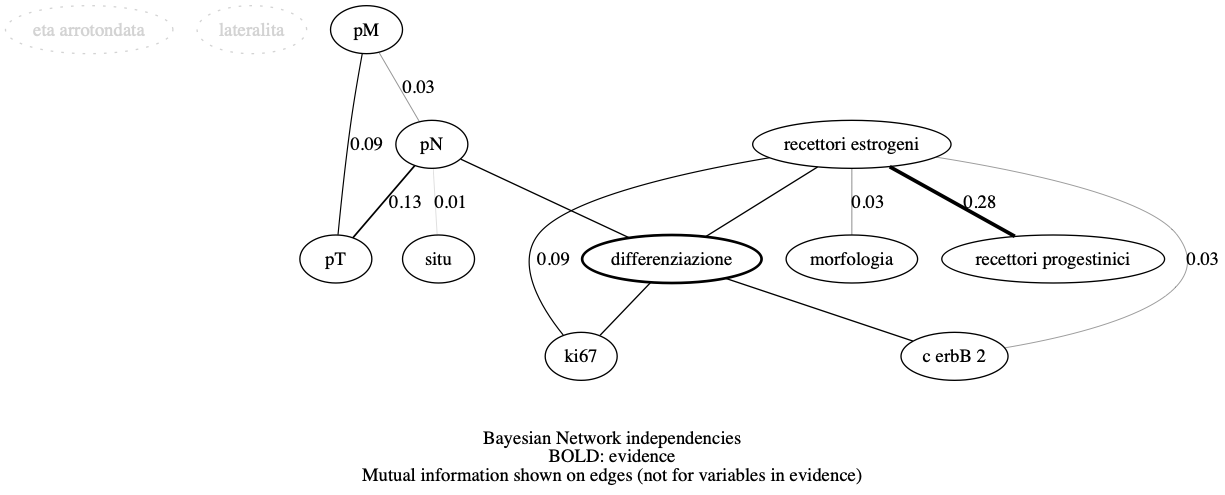
\includegraphics[width=\columnwidth]{methodology/images/example-d-separation-mpe_1}}
\caption{Example output during the first round of the d-separation-aware variant of \texttt{dialogue}.
	The variable \enquote{mut17q21} is the initial evidence.}
\label{fig:pseudo-mpe-independencies_1}
\end{figure}

\begin{figure}[htbp]
\centerline{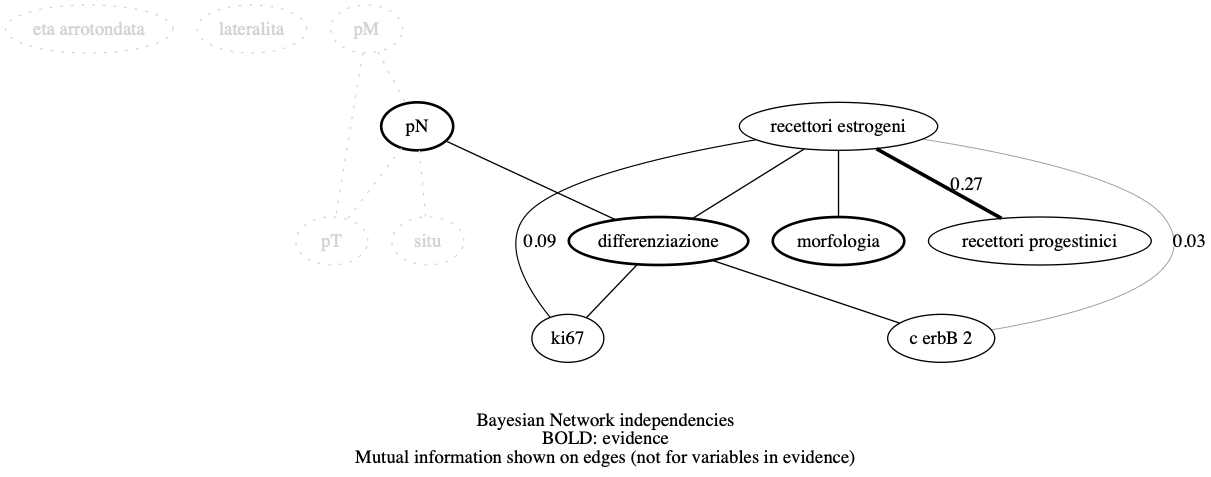
\includegraphics[width=\columnwidth]{methodology/images/example-d-separation-mpe_2}}
\caption{Example output during the second round of the d-separation-aware variant of \texttt{dialogue}.
	\enquote{morfologia} is added to the evidence set and this makes a large part of the network redundant.}
\label{fig:pseudo-mpe-independencies_2}
\end{figure}

\todo{implementare e finire}
\begin{algorithm}[htp!]
	\caption{Thresholded pseudo-MPE algorithm}
	\label{alg:pseudo-mpe-thresholded}
	\begin{algorithmic}
		\STATE $separated\_list = \emptyset$
		\STATE {\bf input:} source $X$, evidence $E$, nodes $V$
		\FOR{target $Y \in V$} 
		\STATE append $d-separated(X, Y, E)$ to $separated\_list$ \COMMENT{will return true or false}
		\ENDFOR
		\STATE {\bf output:} $separated\_list$
	\end{algorithmic}
\end{algorithm} 

\subsubsection{Alternative Explanation Branches}

\subsubsection{\enquote{Pseudo-MPE} from Random Evidence} \label{subsubsec: pseudo-mpe-random}

\subsubsection{Inverse Explanation}
\todo{da fare e trovare nome migliore}

\subsubsection{Natural Language Explanation}
\todo{da fare e magari pensare anche a visual explanations?}

\subsubsection{Pairwise Correlations}
An interesting addition is an algorithm to measure the interrelatedness between pairs of variables.

\subsubsection{Network Plotting} \label{subsubsec:plot-model}

